\section{Background}\label{sec:background}

\subsection{Cloud Computing and Virtualization}

The Cloud infrastructure is typically offered through different virtualization techniques and degrees. It is considered to be a black box: this means that we do not have access to the hypervisor or to
the underlying physical machines. A Cloud instance or \textit{node} is traditionally materialized as a Virtual Machine (VM). However,
nowadays a node might also be a container. Containers provide yet another virtualization technique that operates at the Operating System (OS) level, to create isolated views of the operating environment for different applications. A container has its own process space, virtualized network interface, and file system; and the operating system can allocate different amounts of resources (e.g., CPU, memory, and I/O) to each of them.

Multiple VMs are managed by a single hypervisor that resides on a single host operating system. Each VM then contains its own guest operating system, its own platform stack composed of different libraries, middleware, and application servers, and its own application code. On the other hand, containers are executed directly on top of the host operating system, optionally with the help
of a container manager like Docker\footnote{Docker -- \url{http://docker.com}}. Each container has its own platform stack and its own application code. Containers have various advantages when compared to VMs: they are more lightweight and they are faster to boot and
to terminate because they do not have to deal with a guest
operating system~\cite{FelterContainerVm15,SoletzContainerVirt14}.
%Industry is widely adopting containers as a means to favor portability and they are considered to be one of the main technological enablers of the DevOps movement [36]. Different development teams may use different operating systems and different platform stacks, making feature integration hard. However, thanks to containerization technology, features can be developed in isolation, with the guarantee that they will work the exact same way on any machine that supports containers.


\subsection{Serverless Computing and Functions as a Service}

Serverless Computing is an emerging and compelling paradigm for the deployment of cloud applications, largely due to the recent shift of enterprise application architectures to containers and microservices~\cite{baldini2017serverless}.  A Serverless Architecture is a refined cloud computing model to process requested functionality without pre-allocating any computing capability. Provider-managed containers are used to execute functions (often called lambdas), which are automatically provisioned on demand in few milliseconds, elastically scaled as needed, and ephemeral (may only last for one invocation)~\cite{Roberts:2016}. This approach allows one to write and deploy code without considering the server runtime
environment, resource allocation, load balancing, and scalability; all these aspects are automatically handled by the provider --- hence the term serverless. Functions are charged per invocation and per product of period of time and resource usage (with a millisecond granularity), leading to an almost perfect pay-as-you-go utility pricing model~\cite{MateosFaaster17}.  This allows companies to drastically reduce the cost of their infrastructures with regard to a typical monolithic architecture or even a microservices architecture~\cite{Villamizar2017lambda}.

The Serverless architecture has many benefits with respect to more traditional, server-based approaches. Functions share the runtime environment (typically a pool of containers), and the code specific to a particular application is small and stateless by design. Hence, the deployment of a pool of shared containers (workers) on a machine (or a cluster of machines) and the execution of some code onto any of them becomes inexpensive and efficient. In this manner, the serverless model represents the logical conclusion of the evolution of sharing between applications, from hardware to operating systems to (finally) the runtime environments themselves (Figure~\ref{fig:Evolution-of-Sharing}).

\begin{figure}
  \centering
    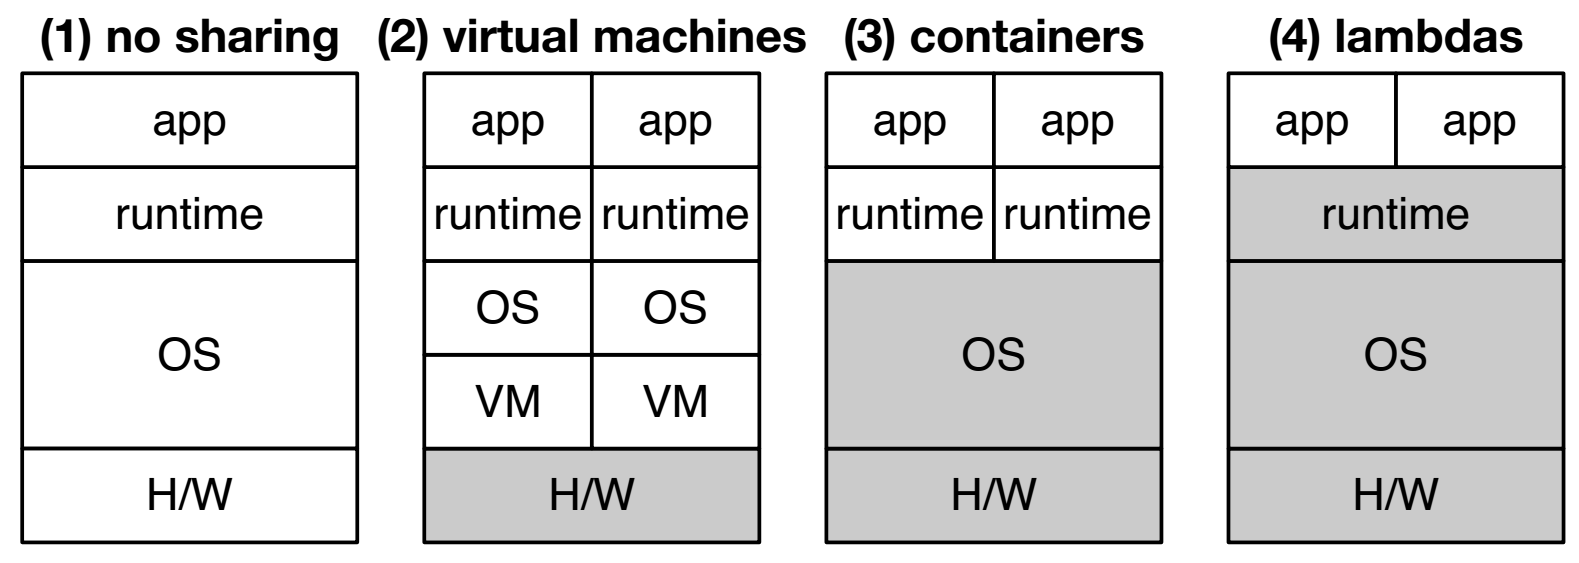
\includegraphics[width=0.7\textwidth]{figs/evolution-platform-sharing.png}    
    \caption{Evolution of platform sharing~\cite{Hendrickson:2016}}
    \label{fig:Evolution-of-Sharing}
\end{figure}


From the everything-as-a-service (XaaS) cloud computing taxonomies point of view, serverless is also known as Function-as-a-Service (FaaS)~\cite{MateosFaaster17}. There is still a controversy regarding how this differs from the Platform-as-a-Service (PaaS) model, which also abstracts away the management of servers. However, a Serverless model is a refinement of the platform layer where, unlike PaaS, developers can write arbitrary code and are not limited to using a pre-packaged application, but explicitly use functions as the deployment unit. 


From the automation point of view, it is important to consider the varying levels of control that the application developer has over the cloud infrastructure, as illustrated in Figure~\ref{fig:developer-control-serverless}. The Infrastructure-as-a-Service (IaaS) model is where less automation is achieved, while the application developer has the most control over both the application code and operating infrastructure. On the opposite extreme are the PaaS and SaaS models, where the developer is unaware of any infrastructure and uses pre-packaged applications and services. Consequently, she no longer has control since the infrastructure provision is completely automated. In the middle, where serverless lives, the application developer has control over the code they deploy into the Cloud, though that code has to be written in the form of stateless functions.  The operational aspects of deployment and maintenance are completely automated, fault-tolerant and
auto-scaling. In particular, the code may be scaled to zero where no servers are actually running when the user's function code is not used, and there is no cost to the user. This is in contrast to PaaS solutions where the user is often charged even during idle periods~\cite{baldini2017serverless}.

\begin{figure}[tbp]
	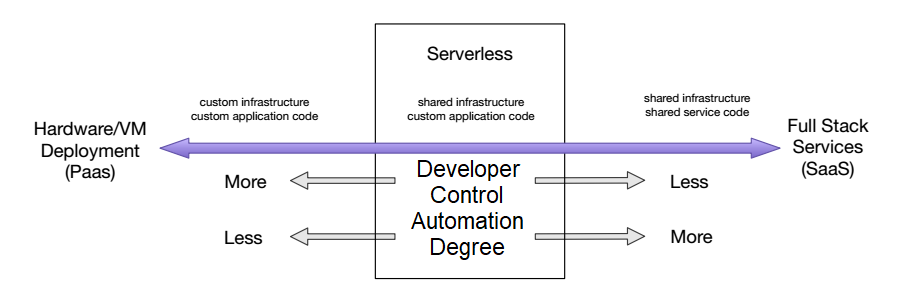
\includegraphics[width=0.9\textwidth]{figs/DeveloperControl.png}
	\caption{Automation degree in the XaaS taxonomy and the situation of serverless computing (adapted from~\cite{baldini2017serverless})}
	\label{fig:developer-control-serverless}
\end{figure}


Finally, from the Cloud providers point of view, serverless represents another revenue opportunity: the provider offers an ecosystem of preexisting services that augment the user's functions. For example, there may be services to manage state, record and monitor logs, send alerts, trigger events, or perform authentication and authorization. Such rich ecosystems can be attractive to developers, leading to an increased adoption of the vendor's solutions. Several cloud providers have developed serverless platforms recently, many of which are still in their explicit or implicit beta testing phase\footnote{\url{https://blog.zhaw.ch/icclab/faas-function-hosting-services-and-their-technical-characteristics}}. Table~\ref{tab:FaaS-providers-and} summarizes the main serverless solutions, with AWS Lambda that appeared 1.5 years before the others (around 2015). All these alternatives provide similar capabilities, while IBM/Apache Openwhisk is the only open-source solution among the major vendors. Other academic alternatives exist, such as OpenLambda\cite{Hendrickson:2016}, but these are mostly suitable for research purposes.

\begin{table}[hbt]
\centering
\caption{Serverless providers and supported languages\label{tab:FaaS-providers-and}}{
\begin{tabular}{ll}
\toprule 
\textbf{Provider} & \textbf{Languages}\tabularnewline
\midrule
AWS Lambda & Node.js, Java, Python\tabularnewline
Google Cloud Functions & Node.js\tabularnewline
Azure Functions & Node.js, C\#\tabularnewline
IBM OpenWhisk & Node.js, Swift, Binary (Docker)\tabularnewline
Webtask.io & Node.js\tabularnewline
OpenLambda & Python\tabularnewline
\bottomrule
\end{tabular}}
\end{table}

%provide what is been called as \textit{Functions as a Service} (FaaS). A FaaS is a realization of the serverless paradigm in which stateless functions  


\subsection{Edge Computing}

Edge computing can be defined by the set of technologies that enable computation to be performed at the network edge~\cite{Shi:2016}. Its main goal is to allow data produced and consumed at the network edge to be processed with low-latency and without overstressing the more centralized cloud infrastructure.

As examples of edge technologies, Cloudlets~\cite{Satyanarayanan:2009} have been first presented as mobile cloud servers that can be positioned at strategic locations to provide computing resources to resource constrained devices with low-latency. 
%with expected high density of users (e.g., at concert halls, stadiums) or areas with temporary infrastructure limitations (e.g., after disasters). 
Additionally, mobile edge computing (MEC)~\cite{ahmed2016isco} relies on cellular infrastructure to enable a low-latency communication between user equipment (i.e., mobile devices) and servers. 

The main motivation for shifting computation from cloud to the network edge is the mitigation of network latency~\cite{Bonomi2014}. In specific, real-time applications are the main candidates for benefiting of services deployed at nearby edge infrastructure. For example, Augmented Reality (AR) is a type of application that would benefit from the low-latency of edge services~\cite{hu2015mobile,GarrigaMendonca2017}. Moreover, mobile devices exhibit limitations that may further motivate the use of edge computing as part of a continuum: some mobile applications rely on heavyweight tasks that can overstress the platform and limit the concurrent execution of other applications; and the battery is a valuable resource that may be significantly affected by the kind of task performed locally~\cite{Carroll:2010}. 

%In addition to the aforementioned types of edge computing, in this paper we explore the usage of \textit{local-edge} as servers deployed as part of a building infrastructure to further improve the computational power of nearby devices. 